\setchapterpreamble[u]{\margintoc}
\chapter{Harmonic Oscilator}

We want to use the algebra we learnt in the previous chaoter, for that we will try to solve the problem where the potential V(x), is a one dimensional harmonic oscilator potential.

\section{Definition}

The potential for an harmonic oscilator in 1 dimension is given by the expresion:

\begin{equation}
  \begin{array}{cc}
    V(x) = \frac{1}{2} k x^2 & k > 0
  \end{array}
\end{equation}

This potential comes from a force, $F(x) = -k x$, so the units of k are kg/s^2. Because of this we can say that:

\begin{equation}
  \omega=\sqrt{\frac{k}{m}}
\end{equation}

Using Newton 3rd Law we can say:

\begin{equation}
  \frac{d^2x}{dt^2}= -\omega^2 x
\end{equation}

Solving this equation we get:

\begin{equation}
  \begin{array}{c}
    x(t) = A \sin(\omega t) + B \cos(\omega t)
    \\
    v(t) = A\omega \cos(\omega t) - B\omega \sin(\omega t)
  \end{array}
\end{equation}

If we define some initial conditions such as $x(0)=x_0$ and $v(0)=0$, we can solve the coeficients, in this case B=x_0 and A=0.

\begin{equation}
  \begin{array}{c}
    x(t) = x_0 \cos(\omega t)
    \\
    v(t) =  - x_0 \omega \sin(\omega t)
  \end{array}
\end{equation}

And we can define two energies, a potential energy and a kinetic energy. The total energy is going to be the addition of the other two.

\begin{equation}
  \begin{array}{c}
    P.E(t) = \frac{1}{2} k (x(t))^2 = \frac{1}{2} k x_0^2 cos^2(\omega t)
    \\
    K:E(t) = \frac{1}{2} m (v(t))^2 = \frac{1}{2} m \omega^2 x_0^2 sin^2(\omega t)
    \\
    T.E(t) = P.E + K.E = \frac{1}{2} k x_0^2 = constant > 0
  \end{array}
\end{equation}

The total energy turn to be constant among time and positive.

\section{Solving the Wave Equation}

The Schrödinger wave equation gets the shape:

\begin{equation}
  \left[\frac{-\hbar^2}{2m}\frac{d^2}{dx^2}+\frac{1}{2}kx^2\right]\phi(x) = E \phi(x)
\end{equation}

Firstly, we will simplify the equation using natural units. We will make a change of variables $x=by$ and try to get the equation for $\phi(bx)=\chi(y)$.

\begin{equation}
  \begin{array}{c}
    \frac{-\hbar^2}{2mb^2}\frac{d^2\chi(y)}{dy^2}+\frac{1}{2}kby^2\chi(y) = E\chi(y)
    \\
    \frac{\hbar^2}{2mb^2} = \frac{1}{2}k b^2
    \\
    b^2 = \frac{\hbar^2}{m\omega}
  \end{array}
\end{equation}

Now that we have the factor to turn into natural units we can rewrite our wave equation. We will also use the definition of the energy given in the second chapter, $E=\hbar \omega$.

\begin{equation}
  \begin{array}{c}
    -\frac{1}{2}\hbar \omega \frac{d^2\chi(y)}{dy^2} + \frac{1}{2} \hbar \omega y^2 \chi(y) = \alpha(\hbar\omega)\chi(y)
    \\
    -\frac{1}{2}\frac{d^2\chi_n}{dy^2}+\frac{1}{2}y^2\chi_n = \alpha_n \chi_n
  \end{array}
\end{equation}

We want to find alpha and it's associate $\chi$. We will define the hermitian operator H from the previous equation.

\begin{equation}
  \begin{array}{c}
    \right[-\frac{1}{2}\frac{d^2}{dy^2}+\frac{1}{2}y^2\left]\chi_n = [\alpha_n] \chi_n
    \\
    H \chi_n = [\alpha_n] \chi_n
  \end{array}
\end{equation}

We define the operator a using what we propose in the end of the previous chapter.

\begin{equation}
  \begin{array}{c}
    a=\frac{1}{\sqrt{2}}\left(\frac{d}{dy}+y\right)
    \\
    a^\dagger = \frac{1}{\sqrt{2}}\left(\left(\frac{d}{dy}\right)^\dagger+(y)^\dagger\right) = \frac{1}{\sqrt{2}}\left(-\frac{d}{dy}+y\right)
    (aa^\dagger)f(y) = \left(-\frac{1}{2}\frac{d^2}{dy^2}+\frac{1}{2}y^2-\frac{1}{2}\right)f(y)
  \end{array}
\end{equation}

We will called $aa^\dagger$ a new operator N, i. e. $N=aa^\dagger$. This operator is hermitian.

\begin{equation}
  \begin{array}{c}
    aa^\dagger - a^\dagger a = \left(-\frac{1}{2}\frac{d^2}{dy^2}+\frac{1}{2}y^2+\frac{1}{2}\right) - \left(-\frac{1}{2}\frac{d^2}{dy^2}+\frac{1}{2}y^2-\frac{1}{2}\right) = 1
  \end{array}
\end{equation}

This resolut is interesting for many reason but one of them is that it prove that a can not be represented as a matrix.

Summarizing what we do so far with this operators:

\begin{equation}
  \begin{array}{c}
    [a,a^\dagger]=1
    \\
    [N,a] = -a
    \\
    [N,a^\dagger] = a^\dagger
  \end{array}
\end{equation}

If we go again to the wave equation we have:

\begin{equation}
  \begin{array}{c}
    [a,a^\dagger+\frac{1}{2}=\alpha]\chi
    \\
    N\chi = \left(\alpha-\frac{1}{2}\right)\chi
    \\
    aN\chi = \left(\alpha-\frac{1}{2}\right)a\chi
    \\
    N[a\chi]=\left(\alpha-1-\frac{1}{2}\right)a\chi
  \end{array}
\end{equation}

$a\chi$ is an eigenvector with eigenvalue $(\alpha-1)$

We can prove that $\chi$ have infinite solutions.

\begin{equation}
  \begin{array}{c}
    a^\dagger N \chi = \left(\alpha - \frac{1}{2}\right)a^{\dagger}\chi
    \\
    (Na^\dagger-a^\dagger) \chi = \left(\alpha - \frac{1}{2}\right)a^{\dagger}\chi
    \\
    N(a^\dagger\chi)=\left(\alpha+1-\frac{1}{2}\right)(a^\dagger\chi)
  \end{array}
\end{equation}

If $\chi$ has finite solutions, a has to be a finite matrix, and we prove that is not allowed.

\begin{equation}
  \int_{-\infty}^{\infty} f*(aa^\dagger f)dx = \int_{-\infty}^{\infty} (af)*(af) dx \geq 0
\end{equation}

Now we know that $\alpha \geq\frac{1}{2}$.

We can search now for our first solution.

\begin{equation}
  \begin{array}{c}
    a\chi_0 = 0 =>
    \\
    => \left(\frac{d}{dy}+\frac{1}{2}\right)\chi_0 = 0
    \\
    \left(aa^\dagger+\frac{1}{2}\right)\chi_0 = \frac{1}{2} \chi_0
  \end{array}
\end{equation}

The first two lines represent the lowest solution and the last one is the next solution. With this we get that:

\begin{equation}
  \alpha = n+\frac{1}{2}
\end{equation}

Now we want to calculate $\chi_0$.

\begin{equation}
  \begin{array}{c}
    N\chi_0 = 0
    \\
    a\chi_0 = 0
    \\
    \chi_0 = \frac{1}{\sqrt{2\pi}}e^{-\frac{y^2}{2}}
  \end{array}
\end{equation}

From this we can say that:

\begin{equation}
  \begin{array}{c}
    N\chi_n = n \chi_n
  \end{array}
\end{equation}

We want to normalize $\chi_n$ so we will ad a normalization factor C, where $a^\dagger\chi_n=C\chi_{n+1}$

\begin{equation}
  \begin{array}{c}
    C^2 \int_{-\infty}^{\infty} \chi^2_{n+1} dy = \int_{-\infty}^{\infty} (a^\dagger\chi_n)(a^\dagger\chi_n)dy = \int_{-\infty}^{\infty} =
    \\

    \\
    = \int_{-\infty}^{\infty}\chi_n(aa^\dagger\chi_n)dy=\int_{-\infty}^{\infty}\chi_n n\chi_n dy + \int_{-\infty}^{\infty}\chi_n^2dy= n+1
    \\

    \\
    C = \sqrt{n+1}
  \end{array}
\end{equation}

We want to redifine $\chi_n$ as:

\begin{equation}
  \chi_n = \frac{H_n(y)}{\sqrt{2\pi}}e^{\frac{-y^2}{2}}
\end{equation}

We want to find H_{n+1} using the previous two equations.

\begin{equation}
  \begin{array}{c}
    a^\dagger \chi_n = C \chi_{n+1} = \sqrt{1+n} \chi_{n+1}
    \\

    \\
    \frac{1}{\sqrt{2}}\left(-\frac{d}{dx}+y\right)\frac{H_n(y)}{\sqrt{2\pi}}e^{\frac{-y^2}{2}} = \sqrt{n+1} \frac{H_{n+1}}{\sqrt{2\pi}}e^{\frac{-y^2}{2}}
    \\

    \\
    \frac{1}{\sqrt{2(n+1)}}\left[-H'(y)e^{\frac{-y^2}{2}}+y H(y)e^\frac{-y^2}{2}+y H(y)e^\frac{-y^2}{2}\right]= H_{n+1} e^\frac{-y^2}{2}
    \\

    \\
    H_{n+1} = \frac{1}{\sqrt{2(n+1)}}\left[-H_n'(y)+2 y H_n(y)\right]
  \end{array}
\end{equation}

Whre $H_0$ is define as $H_0=1$.

Because $\chi_n$ is normalized we can say that $H_n(y)$ are orthonormal polynomials under a Gaussian width.

\begin{equation}
  \begin{array}{c}
    \frac{1}{2\pi}\int_{-\infty}^{\infty} \chi_n(y) \chi_m(y) dy = \delta_{nm}
    \\

    \\
    \frac{1}{2\pi}\int_{-\infty}^{\infty} H_n(y) H_m(y) e^{\frac{-y^2}{2}}dy = \delta_{nm}
  \end{array}
\end{equation}

We called this functions Hermite polynomials.

\begin{figure}[H]
  \centering
  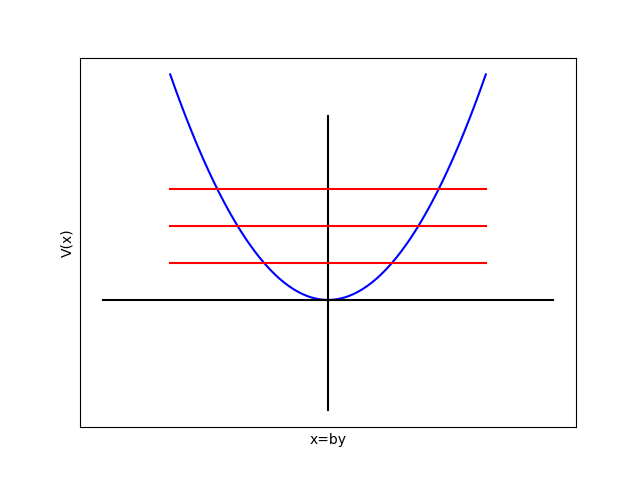
\includegraphics{images7/sol.png}
  \caption{Potential V(x) and some energy levels.}
\end{figure}

We can see the solution for the problem in the figure above, where the distance of the gaps between the energies is always $\hbar\omega$.


\section{Temperature}

We have solved our potential, but we want to think now about a problem wiht multiple of this potentials. Firstly, we assume we are talking about an ideal gas wich means the particles don't talk one with each others. We want to answer the question; At a temperature, T what is the probablity that the energy is $\left(n+\frac{1}{2}\right)\omega$

We want to relate $K_b T <-> \left(n+\frac{1}{2}\right)\omega$. We have Boltzmann equation that say:

\begin{equation}
  P_n = Ne^{\frac{-(n+1/2)\hbar\omega}{k_B T}}
\end{equation}

It is a negative exponential where the fall of depend on T

Because it is a probablity for a fixed N we should have $\sum_{n=0}^{N}P_n = 1$ when N goes to $\infty$.

The average energy, E, will be define as:

\begin{equation}
  E = \sum_{n=0}^{\infty}E_nP_n
\end{equation}

If we called $\beta = \hbar\omega/k_B T$ we can get the average energy as:

\begin{equation}
  \frac{E}{k_B T} = \frac{\beta(1+e^{-\beta})}{2(1-e^{-\beta})}
\end{equation}

The behaviour of this function can be seen in the plot below.


\begin{figure}[H]
  \centering
  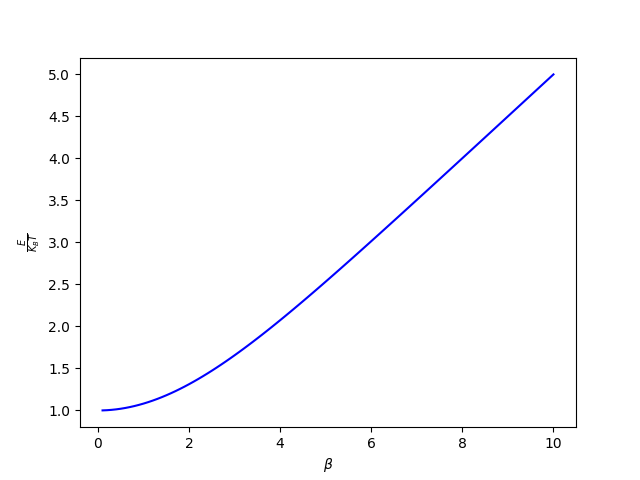
\includegraphics{images7/E_beta.png}
  \caption{Potential V(x) and some energy levels.}
\end{figure}

If T goes to infinite the average energy goes to $E=K_BT$ and if T goes to 0 the average energy goes to $E=\frac{\hbar\omega}{2}$.

We will retur to the topic of temperature in future chapters.
